\begin{titlepage}


%\begin{center}
%\begin{tabular}{r c}
%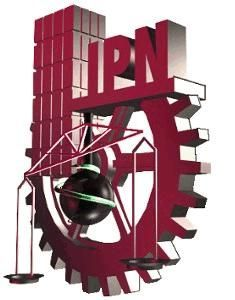
\includegraphics[scale=.3]{images/ipn.jpg} & \LARGE \textbf{Instituto Polit\'ecnico Nacional} & 
\includegraphics[scale=.3]{images/escom.jpg} \\
%& \Large \textbf{Escuela Superior de C\'omputo} &
%\end{tabular}
%\end{center}

\begin{center}
\begin{tabular}{r c l}
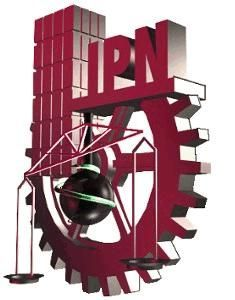
\includegraphics[scale=.25]{images/ipn.jpg} & \huge \textbf{INSTITUTO POLIT\'ECNICO NACIONAL} & 
\includegraphics[scale=.25]{images/escom.jpg}\\ 
& \Large \textbf{ESCUELA SUPERIOR DE C\'OMPUTO}
\end{tabular}
\end{center}


\vspace{1.5cm}
\begin{center}
\large Trabajo Terminal: \linebreak

\large \textbf{``Sistema de identificaci\'on de art\'iculos utilizando reconocimiento de patrones.''} \linebreak
\large 2015B-032

\end{center}

\vspace{1.5cm}

\begin{center}
Presentan: \linebreak
\textbf{Calvillo Ju\'arez Rogelio} \linebreak
\textbf{Casta\~neda Vite Carlos Rodrigo} \linebreak
\textbf{Mej\'ia Hern\'andez Miguel} \linebreak
\end{center}

\vspace{1.5cm}


En el presente documento se encuentran los resultados correspondientes al desarrollo del Trabajo Terminal cuyo objetivo es la implementaci\'on de un sistema que analice im\'agenes mediante  el procesamiento de las mismas . Este sistema pretende servir como herramienta capaz \linebreak

\textbf{Palabras Clave}:  Reconocimiento de patrones,  procesamiento de im\'agenes, inteligencia artificial, aprendizaje máquina, aplicaci\'on web.

\vspace{1.5cm}
 
\begin{center}


Directores: \linebreak
\textbf{ M. en C. Ram\'irez Morales Mario Augusto, M. en E.  Silva S\'anchez Carlos}

\end{center}





\end{titlepage}
